\documentclass{article}

\usepackage{fancyhdr}
\usepackage{extramarks}
\usepackage{amsmath}
\usepackage{amsthm}
\usepackage{amsfonts}
\usepackage{tikz}
\usepackage[plain]{algorithm}
\usepackage{algpseudocode}
\usepackage{graphicx}
\usepackage{gensymb}
\usepackage[framed,numbered,autolinebreaks,useliterate]{mcode}
\usepackage{listings}

\graphicspath{{./images/}}

\usetikzlibrary{automata,positioning}

%
% Basic Document Settings
%

\topmargin=-0.45in
\evensidemargin=0in
\oddsidemargin=0in
\textwidth=6.5in
\textheight=9.0in
\headsep=0.25in

\linespread{1.1}

\pagestyle{fancy}
\lhead{\hmwkAuthorName}
\chead{\hmwkClass\ \hmwkTitle}
\rhead{\firstxmark}
\lfoot{\lastxmark}
\cfoot{\thepage}

\renewcommand\headrulewidth{0.4pt}
\renewcommand\footrulewidth{0.4pt}

\setlength\parindent{0pt}

%
% Create Problem Sections
%

\newcommand{\enterProblemHeader}[1]{
    \nobreak\extramarks{}{Problem {#1} continued on next page\ldots}\nobreak{}
    \nobreak\extramarks{{#1} (continued)}{{#1} continued on next page\ldots}\nobreak{}
}

\newcommand{\exitProblemHeader}[1]{
    \nobreak\extramarks{{#1} (continued)}{{#1} continued on next page\ldots}\nobreak{}
    % \stepcounter{#1}
    \nobreak\extramarks{{#1}}{}\nobreak{}
}

\setcounter{secnumdepth}{0}
\newcounter{partCounter}

\newcommand{\problemNumber}{0.0}

\newenvironment{homeworkProblem}[1][-1]{
    \renewcommand{\problemNumber}{{#1}}
    \section{\problemNumber}
    \setcounter{partCounter}{1}
    \enterProblemHeader{\problemNumber}
}{
    \exitProblemHeader{\problemNumber}
}

%
% Homework Details
%   - Title
%   - Class
%   - Author
%

\newcommand{\hmwkTitle}{Homework\ \#4}
\newcommand{\hmwkClass}{RBE 500}
\newcommand{\hmwkAuthorName}{\textbf{Arjan Gupta}}

%
% Title Page
%

\title{
    \vspace{2in}
    \textmd{\textbf{\hmwkClass\ \hmwkTitle}}\\
    \vspace{3in}
}

\author{\hmwkAuthorName}
\date{}

\renewcommand{\part}[1]{\textbf{\large Part \Alph{partCounter}}\stepcounter{partCounter}\\}

%
% Various Helper Commands
%

% Useful for algorithms
\newcommand{\alg}[1]{\textsc{\bfseries \footnotesize #1}}

% For derivatives
\newcommand{\deriv}[2]{\frac{\mathrm{d}}{\mathrm{d}#2} \left(#1\right)}

% For compact derivatives
\newcommand{\derivcomp}[2]{\frac{\mathrm{d}#1}{\mathrm{d}#2}}

% For partial derivatives
\newcommand{\pderiv}[2]{\frac{\partial}{\partial #2} \left(#1\right)}

% For compact partial derivatives
\newcommand{\pderivcomp}[2]{\frac{\partial #1}{\partial #2}}

% Integral dx
\newcommand{\dx}{\mathrm{d}x}

% Alias for the Solution section header
\newcommand{\solution}{\textbf{\large Solution}}

% Probability commands: Expectation, Variance, Covariance, Bias
\newcommand{\E}{\mathrm{E}}
\newcommand{\Var}{\mathrm{Var}}
\newcommand{\Cov}{\mathrm{Cov}}
\newcommand{\Bias}{\mathrm{Bias}}

\begin{document}

\maketitle

\nobreak\extramarks{Problem 4.6}{}\nobreak{}

\pagebreak

\begin{homeworkProblem}[Problem 4.6]
    Given \(R = R_{x,\theta}R_{y,\phi}\), compute \(\pderivcomp{R}{\phi}\).
    Evaluate \(\pderivcomp{R}{\phi}\) at $\theta = \frac{\pi}{2}$, $\phi = \frac{\pi}{2}$.
    First parametrically compute, then evaluate by plugging the values in. 

    \subsection{Solution}

    \[
        \pderiv{R_{x,\theta}R_{y,\phi}}{\phi} = R_{x,\theta}\pderiv{R_{y,\phi}}{\phi}
    \]
    Using the the fact that \(\deriv{R_{y,\theta}}{\theta} = S(j)R_{y,\theta}\),
    \begin{align*}
        R_{x,\theta}\pderiv{R_{y,\phi}}{\phi} =
        R_{x,\theta}S(j)R_{y,\phi}
        &=
        \begin{bmatrix}
            1 & 0 & 0\\
            0 & \cos\theta & -\sin\theta\\
            0 & \sin\theta & \cos\theta
        \end{bmatrix}   
        \begin{bmatrix}
            0 & 0 & 1\\
            0 & 0 & 0\\
            -1 & 0 & 0
        \end{bmatrix}
        \begin{bmatrix}
            \cos\phi & 0 & \sin\phi\\
            0 & 1 & 0\\
            -\sin\phi & 0 & \cos\phi
        \end{bmatrix}\\
        &= \begin{bmatrix}-\sin\left(\phi \right) & 0 & \cos\left(\phi \right)\\ \cos\left(\phi \right)\,\sin\left(\theta \right) & 0 & \sin\left(\phi \right)\,\sin\left(\theta \right)\\ -\cos\left(\phi \right)\,\cos\left(\theta \right) & 0 & -\cos\left(\theta \right)\,\sin\left(\phi \right)\end{bmatrix}
    \end{align*}
    Now, plugging in the values $\theta = \frac{\pi}{2}$, $\phi = \frac{\pi}{2}$, we get
    \[
        \begin{bmatrix}
            -1 & 0 & 0\\
            0 & 0 & 1\\
            0 & 0 & 0
        \end{bmatrix}
    \]
    \vspace{0.2in}
    \\We performed the above computations using the following MATLAB code.
    \lstinputlisting{./prob4_6.m}
    
\end{homeworkProblem}

\nobreak\extramarks{Problem 4.10}{}\nobreak{}

\pagebreak

\begin{homeworkProblem}[Problem 4.10]
    Two frames $o_0x_0y_0z_0$ and $o_1x_1y_1z_1$ are related by the homogeneous transformation

    \[
        H =
        \begin{bmatrix}
            0 & -1 & 0 & 1\\
            1 & 0 & 0 & -1\\
            0 & 0 & 1 & 0\\
            0 & 0 & 0 & 1
        \end{bmatrix}
    \]

    A particle has velocity $v_1(t) = (3,1,0)$ relative to frame $o_1x_1y_1z_1$. What is the
    velocity of the particle in frame $o_0x_0y_0z_0$?

    \subsection{Solution}

    The given H is the homogeneous transformation $H^0_1$. Therefore, \(
        R^0_1 =
        \begin{bmatrix}
            0 & -1 & 0\\
            1 & 0 & 0\\
            0 & 0 & 1
        \end{bmatrix}
    \) and \(
        o^0_1 =
        \begin{bmatrix}
            1\\
            -1\\
            0
        \end{bmatrix}
    \).
    \vspace{0.15in}
    \\
    At any given point in time, the position of the particle with respect to frame $o_1x_1y_1z_1$ is given as $p^1(t)$.
    We know that

    \[
        p^0(t) = R^0_1 p^1(t) + o^0_1
    \]

    Taking the derivative of both sides and using the product rule, we get

    \[
        v^0(t) = \dot{R^0_1} p^1(t) +  R^0_1 v^1(t) + 0
    \]

    But, $\dot{R^0_1} = 0$ since $R^0_1$ is a constant in time. Therefore,

    \begin{align*}
        v^0(t) &= R^0_1 v^1(t)\\
        v^0(t) &=
            \begin{bmatrix}
                0 & -1 & 0\\
                1 & 0 & 0\\
                0 & 0 & 1
            \end{bmatrix}
            \begin{bmatrix}
                3\\
                1\\
                0
            \end{bmatrix}\\
        v^0(t) &= 
            \begin{bmatrix}
                -1\\
                3\\
                0        
            \end{bmatrix}
    \end{align*}

    Which was calculated by the following MATLAB script

    \lstinputlisting{prob4_10.m}

\end{homeworkProblem}

\nobreak\extramarks{Problem 4.15}{}\nobreak{}

\pagebreak

\begin{homeworkProblem}[Problem 4.15]
    Find the $6 \times 3$ Jacobian for the three links of the cylindrical manipulator of Figure 3.7.
    Find the singular configurations for this arm.

    \subsection{Solution}

    Figure 3.7 of our book is the following.
    \begin{figure}[h]
        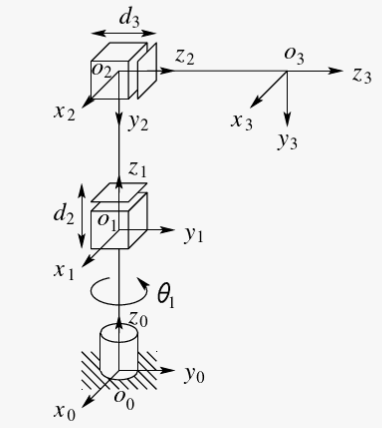
\includegraphics[scale=0.5]{prob4_15.png}
        \centering
    \end{figure}

    We can see that we have 3 joints, so $n = 3$. Let us also form the table given in the lecture videos:

    \begin{table}[h!]
        \begin{center}
            \begin{tabular}{|c|c|c|}
            \hline
            & Linear component & Angular component\\
            \hline
            Revolute joint & \(J_{v_i} = z^0_{i-1} \times (o^0_n - o^0_{i-1})\) & \(J_{v_i} = z^0_{i-1}\) \\
            Prismatic joint & \(J_{\omega_i} = z^0_{i-1}\) & \(J_{\omega_i} = 0\)\\
            \hline
            \end{tabular}
        \end{center}
    \end{table}
    
    Using this table, and the fact that the upper half of the Jacobian contains linear components while the bottom half
    contains angular components, we have
    \[
        J =
        \begin{bmatrix}
           z_0 \times (o_3 - o_0) & z_1 & z_2\\
           z_0 & 0 & 0
        \end{bmatrix}
    \]

    In this Jacobian matrix, we know that \(z_0 = \begin{bmatrix}
        0\\
        0\\
        1
    \end{bmatrix}\) and \(o_0 =\begin{bmatrix}
        0\\
        0\\
        0
    \end{bmatrix}\). To find $z_1$, $z_2$, and $o_3$, we need to find
    $T^0_n = A_1 \dots A_n$ for $n = 1, 2, 3$. Following the DH convention
    (which Figure 3.7 already abides by), we have the following table for
    quantities \(\alpha_i, a_i, \theta_i, d_i\).

    \begin{table}[h!]
        \begin{center}
            \begin{tabular}{|c|c|c|c|c|}
            \hline
            Link & $\alpha_i$ & $a_i$ & $\theta_i$ & $d_i$ \\
            \hline
            1 & 0 & 0 & $\theta_1$ & $d_1$ \\
            2 & -90\degree & 0 & 0 & $d_2$\\
            3 & 0 & 0 & 0 & $d_3$\\
            \hline
            \end{tabular}
        \end{center}
    \end{table}

    Which gives us the following $A_i$ matrices.

    \[
        A_1 =
        \begin{bmatrix}\cos\left(\theta _{1}\right) & -\sin\left(\theta _{1}\right) & 0 & 0\\ \sin\left(\theta _{1}\right) & \cos\left(\theta _{1}\right) & 0 & 0\\ 0 & 0 & 1 & d_{1}\\ 0 & 0 & 0 & 1 \end{bmatrix},
    % \]
    % \[
        A_2 =
        \begin{bmatrix}1 & 0 & 0 & 0\\ 0 & 0 & 1 & 0\\ 0 & -1 & 0 & d_{2}\\ 0 & 0 & 0 & 1\end{bmatrix},
        A_3 =
        \begin{bmatrix}1 & 0 & 0 & 0\\ 0 & 1 & 0 & 0\\ 0 & 0 & 1 & d_{3}\\ 0 & 0 & 0 & 1\end{bmatrix}
    \]

    Now we can compute our $T$ matrices using the following MATLAB code,

    \lstinputlisting{prob4_15_tmats.m}

    \[
        T^0_1 = A_1 =
        \begin{bmatrix}\cos\left(\theta _{1}\right) & -\sin\left(\theta _{1}\right) & 0 & 0\\ \sin\left(\theta _{1}\right) & \cos\left(\theta _{1}\right) & 0 & 0\\ 0 & 0 & 1 & d_{1}\\ 0 & 0 & 0 & 1 \end{bmatrix}
    \]
    \[
        T^0_2 = A_1 A_2 =
        \begin{bmatrix}\cos\left(\theta _{1}\right) & 0 & -\sin\left(\theta _{1}\right) & 0\\ \sin\left(\theta _{1}\right) & 0 & \cos\left(\theta _{1}\right) & 0\\ 0 & -1 & 0 & d_{1}+d_{2}\\ 0 & 0 & 0 & 1\end{bmatrix}
    \]
    \[
        T^0_3 = A_1 A_2 A_3 =
        \begin{bmatrix}\cos\left(\theta _{1}\right) & 0 & -\sin\left(\theta _{1}\right) & -d_{3}\,\sin\left(\theta _{1}\right)\\ \sin\left(\theta _{1}\right) & 0 & \cos\left(\theta _{1}\right) & d_{3}\,\cos\left(\theta _{1}\right)\\ 0 & -1 & 0 & d_{1}+d_{2}\\ 0 & 0 & 0 & 1\end{bmatrix}
    \]

    From these $T$ matrices, we get

    \[
        z_1 =
        \begin{bmatrix}
            0\\
            0\\
            1
        \end{bmatrix},
        z_2 =
        \begin{bmatrix}
            -\sin\left(\theta _{1}\right)\\
            \cos\left(\theta _{1}\right)\\
            0
        \end{bmatrix},
        o_3 =
        \begin{bmatrix}
            -d_{3}\,\sin\left(\theta _{1}\right)\\
            d_{3}\,\cos\left(\theta _{1}\right)\\
            d_{1}+d_{2}
        \end{bmatrix}
    \]\\
    \vspace{0.15in}\\

    Now we are ready to compute our Jacobian matrix. We do this using the following
    MATLAB code.

    \lstinputlisting{prob4_15_jacobian.m}

    Which gives us the following Jacobian,

    \[
        J =
        \begin{bmatrix} -d_{3}\,\cos\left(\theta _{1}\right) & 0 & -\sin\left(\theta _{1}\right)\\ -d_{3}\,\sin\left(\theta _{1}\right) & 0 & \cos\left(\theta _{1}\right)\\ 0 & 1 & 0\\ 0 & 0 & 0\\ 0 & 0 & 0\\ 1 & 0 & 0 \end{bmatrix}
        = J_P
        = \left[\begin{array}{@{}c@{}}
            J_{11}\\\hline
            J_{21} \\
            \end{array}\right]
    \]
    Where $J_{11}$ and $J_{21}$ are $3 \times 3$ matrices. By setting $\det J_{11} = 0$ we
    can find the singularity configurations for the arm portion of the manipulator (first
    three joints).
\end{homeworkProblem}

\end{document}